\documentclass[12pt]{article}

\usepackage[utf8]{inputenc}
\usepackage[english]{babel}
\usepackage{natbib}
\usepackage[T1]{fontenc}
\usepackage{setspace}
\usepackage{graphicx}
\usepackage{hyperref}
\usepackage{float}


\graphicspath{ {images/} }

\title{\vspace{1cm}\textbf{Enterprise Programming}\\6G6Z1103}
\author{Joshua Michael Ephraim Bridge\\14032908\\joshua.m.bridge@stu.mmu.ac.uk}

\pagestyle{headings}

\begin{document}

\maketitle

\tableofcontents

\section{Completed Tasks}
  \subsection{HTTP Web Service}
    \begin{figure}[H]
      \centering
      \includegraphics[width=9cm]{http-web-service}
      \caption{Http web service call}
      \label{fig:http-web-service}
    \end{figure}

  \subsection{Data formats}
    For JSON see figure \ref{fig:http-web-service}.

    \begin{figure}[H]
      \centering
      \includegraphics[width=9cm]{http-service-xml}
      \caption{XML web service call}
      \label{fig:http-service-xml}
    \end{figure}

    \begin{figure}[H]
      \centering
      \includegraphics[width=9cm]{http-service-text}
      \caption{TEXT web service call}
      \label{fig:http-service-text}
    \end{figure}

  \subsection{Appengine}
    \begin{figure}[H]
      \centering
      \includegraphics[width=9cm]{appengine-config}
      \caption{Appengine config}
      \label{fig:appengine-config}
    \end{figure}

    \begin{figure}[H]
      \centering
      \includegraphics[width=9cm]{appengine-deployment}
      \caption{Appengine Deployment (\url{http://rest-films.appspot.com})}
      \label{fig:appengine-deployment}
    \end{figure}

    \begin{figure}[H]
      \centering
      \includegraphics[width=9cm]{datastore-entries}
      \caption{Datastore entries}
      \label{fig:datastore-entries}
    \end{figure}

  \subsection{WSDL}
    I could not find a way to convert my java classes to WSDL, I tried it in multiple applications and it never worked. Every example given in the lab exercises was for a SOAP webservice so as my project is mainly a REST service, a WSDL does not seem to apply to it.

  \subsection{REST}
    \begin{figure}[H]
      \centering
      \includegraphics[width=9cm]{rest-create}
      \caption{Film resource create (201 Response - with resource location)}
      \label{fig:rest-create}
    \end{figure}

    \begin{figure}[H]
      \centering
      \includegraphics[width=9cm]{rest-response}
      \caption{Film resource response}
      \label{fig:rest-response}
    \end{figure}

    \begin{figure}[H]
      \centering
      \includegraphics[width=9cm]{rest-update}
      \caption{Film resource update (200 Response)}
      \label{fig:rest-update}
    \end{figure}

    \begin{figure}[H]
      \centering
      \includegraphics[width=9cm]{rest-delete}
      \caption{Film resource deletion (200 Response)}
      \label{fig:rest-delete}
    \end{figure}

  \subsection{AJAX Front-end}
    See figure \ref{fig:appengine-deployment}.

\section{Design Patterns}

  \subsection{Model-view-controller (MVC)}
    The Model-view-controller \citep{krasner1988description} design pattern is one of the most commonly used methods for web development. It has become so essential due to its simplicity, and how it easily separates concerns from different sections of a program. For example a controller class should not have to worry about how to retrieve data from a table - as that is not part of its purpose and will only make the class harder to comprehend and work with. With clear separation of concerns, development in any language or platform becomes a lot simpler. I have used the MVC pattern in my assignment as it was the obvious choice for a simple requirement of displaying film data. However, I did not use the ‘view’ portion of the pattern as the main component was an API returning JSON, XML and TEXT data - and instead of rendering JSP pages I used the Controller itself to render the responses. To do this I used a framework called Spring MVC (see section \ref{spring-mvc}).

  \subsection{Data Access Object (DAO)}
    Data access objects are a very fundamental design pattern which provides access to external services such as database connections or a connection to an external API. In my application I have used the DAO pattern to connect to Google Datastore (a type of NoSql database).

  \subsection{Singleton}
    The Singleton design pattern is used by default in a Spring bean. For example, a class annotated with ‘@Component’ is instantiated and held in the Spring context as a single instance of that class. Whenever you want to use this object you can simply wire it into other fields using the ‘@Autowired’ annotation as shown in figure \ref{fig:spring-autowired-components}. This pattern removes a lot of the hassle for managing different instances of classes, especially as in this situation where multiple instances of controllers and DAO's are not needed so was very effective in my application.

  \subsection{Static Factory}
    I have used a static factory in my application (as seen in figure \ref{fig:static-factory}). Static factories serve to make code more readable when instantiating objects. This can be seen in figure \ref{fig:static-factory-usage} where a Results object is created, and the code actually reads like a sentence - making it much easier to understand what is happening without spending too much time trying to read through it.

    \begin{figure}[ht]
      \centering
      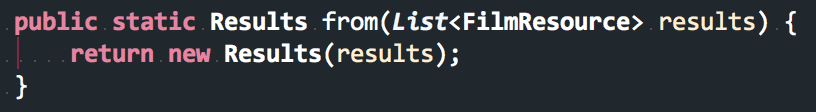
\includegraphics[width=9cm]{static-factory}
      \caption{Static factory method}
      \label{fig:static-factory}
    \end{figure}

    \begin{figure}[ht]
      \centering
      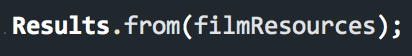
\includegraphics[width=9cm]{static-factory-usage}
      \caption{Static factory method usage}
      \label{fig:static-factory-usage}
    \end{figure}

\section{Refactoring}
  Refactoring is an essential part of developing - especially in a team - in order to make sure your code is easily readable and maintainable. This is especially necessary in a team as other people will often be looking at your code, therefore if it is too difficult to understand then it wastes developers time and money trying to understand it rather than extending it.

  One of the best ways to ensure readable code is to make sure methods and classes only have a single purpose. As shown in figure \ref{fig:film-controller-utilities}, my FilmController class has a set of private utility methods which handle common tasks such as converting a Film object into a web resource (FilmResource). These methods are easy to understand as they only perform a single purpose, and the naming of the methods should make it understandable enough that even if the contents of the method are not understandable, then it's purpose still is clear and the code can still easily be maintained.

  An extension of this is to try and stick to 3 line functions (at least 3 meaningful lines). This is a useful technique as it helps maintain low complexity in any code and ensures an application is split up into meaningful section, which also can be seen in figure \ref{fig:film-controller-utilities}.

  \begin{figure}[ht]
    \centering
    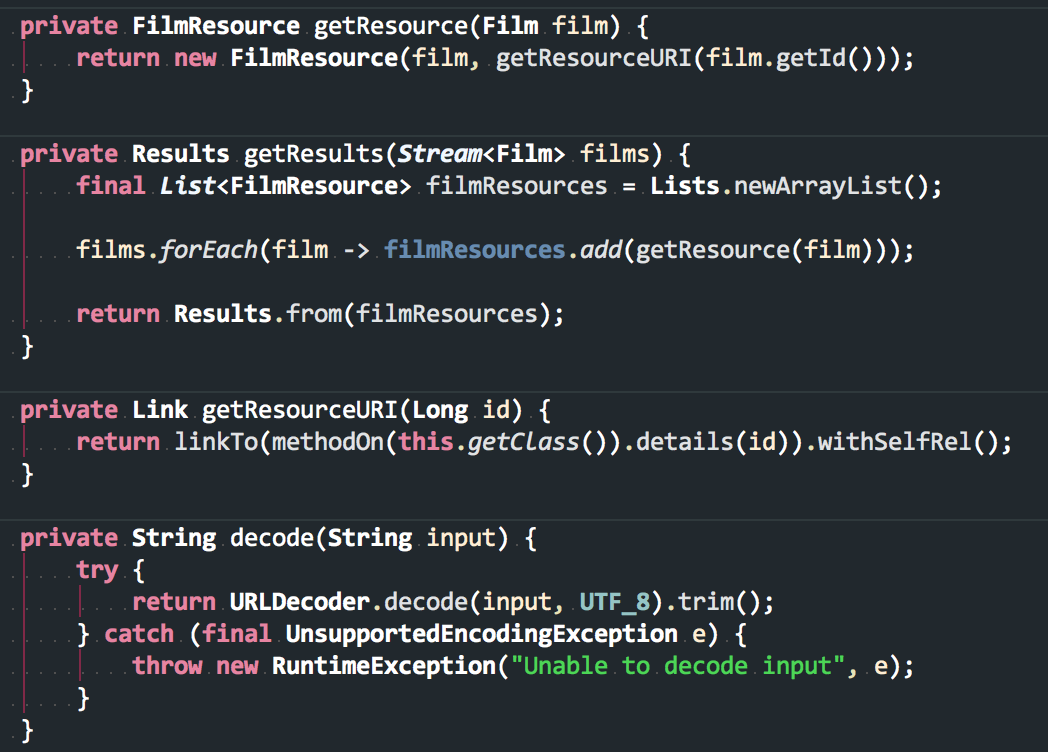
\includegraphics[width=9cm]{film-controller-utilities}
    \caption{Film controller utility methods}    \label{fig:film-controller-utilities}
  \end{figure}

  In figure \ref{fig:film-methods} you can see the getter/setter methods on the Film class, and I have removed the setter methods for everything except from setID. This is due to the fact that originally the fields were immutable, however as explained in \ref{objectify} I had to remove this for multiple reasons. I decided not to add setters for the rest as there was no code that needed them so it would have been pointless, and would have just cluttered up the code.

  \begin{figure}[ht]
    \label{fig:film-methods}
    \centering
    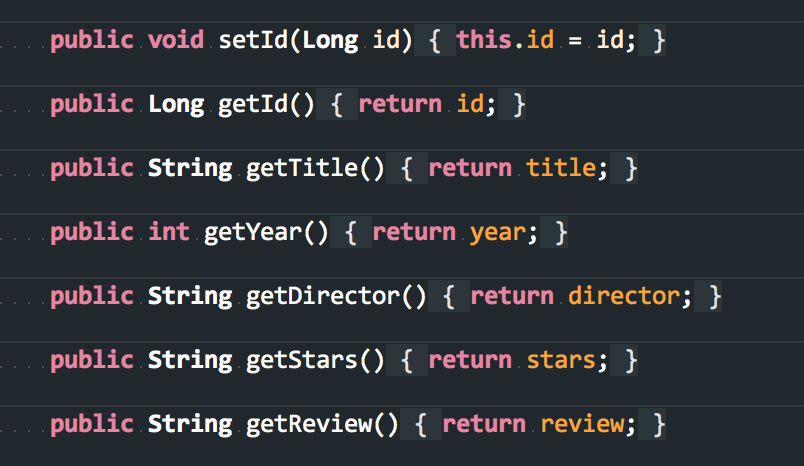
\includegraphics[width=9cm]{film-methods}
    \caption{Film class methods}
  \end{figure}

\section{Libraries (\& Tools)}
  In this section I will talk a little about each of the main third-party libraries I used, why I chose to use them, and how it helped me solve a problem I was facing - or how it reduced reliance on custom code. Reducing as much custom code as possible (in general) is always good as it means you don't have to maintain it yourself and also test it yourself.

  \subsection{Maven}
    While Maven (\url{http://maven.apache.org}) is not technically a library (more a build automation/project management tool), it does come under the umbrella of tools which helped implement a solution. Another well-known tool like this is Gradle (\url{https://gradle.org}), however this is often used for more complex build management which wasn't really what I needed. I only really needed dependency management within this project as there were a lot of dependencies, and Maven is a lot simpler to set up for this task. Without dependency management I would've had to download individual ‘.jar’ files for each library (which each have their own dependencies to download) and manage them across different computers when developing or testing on other machines. It is also a lot easier to change the version of a dependency if there are compatibility issues between different libraries which rely on each other. Finally as my project was developed in git (\url{https://git-scm.com}), dependency management meant I did not have to host large jar files in the repository.

  \subsection{Spring MVC}
    \label{spring-mvc}
    When developing pretty much any Java application, Spring (\url{https://projects.spring.io/spring-framework/}) is an obvious and hugely popular choice for making developing a lot simpler and more focused on business logic than things like dependency injection. Spring MVC is a part of the framework which focuses on web serving applications traditionally using the MVC structure. Spring MVC allows a REST \citep{fielding2000architectural} service to be easily configured, which just serves string data to the page without needing to pass it into a JSP. Spring in general allows for much simpler code to be produced as it handles most of the finicky tasks in java that often just waste time. Fulfilling dependencies is the most common (and most useful) part and allows you to focus on more important tasks.

    \begin{figure}[ht]
      \centering
      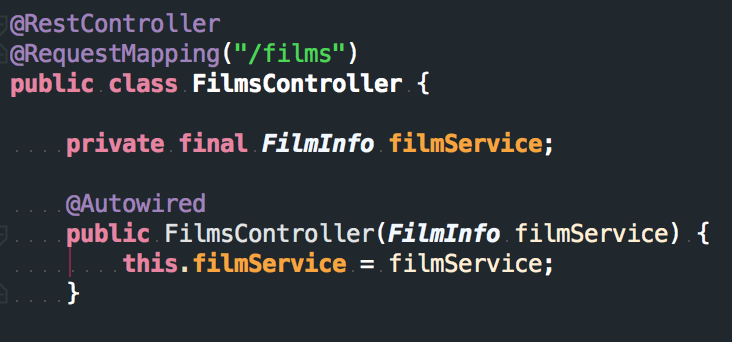
\includegraphics[width=9cm]{autowired-components}
      \caption{Spring's automatic dependency injection}
      \label{fig:spring-autowired-components}
    \end{figure}

    Spring MVC also handles the difficult parts of web service hosting. For example it can handle the response type headers and conversion with no code needed. In the config you can set up which response types you want to allow and how to choose between them and set a default. My config (figure \ref{fig:response-format-config}) allows a ‘?format=json’ parameter to be put after any url in the servlet, and it will convert to that format no matter which endpoint is being accessed.

    \begin{figure}[ht]
      \centering
      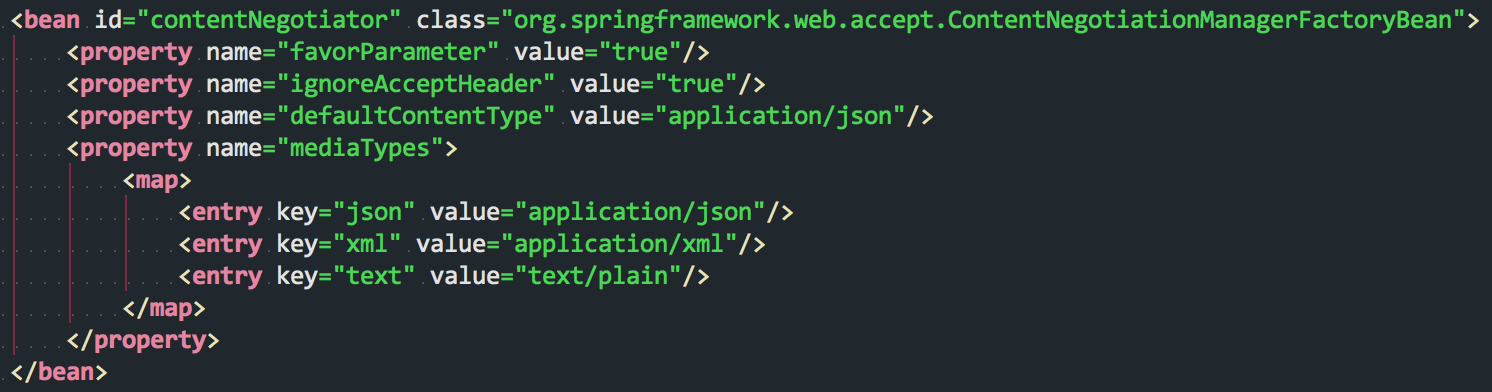
\includegraphics[width=9cm]{response-format-config}
      \caption{Response format spring configuration}
      \label{fig:response-format-config}
    \end{figure}

  \subsection{Spring HATEOAS}
    Spring HATEOAS (\url{http://projects.spring.io/spring-hateoas/}) is a library that extends a lot of Spring MVC functionality to provide REST representations of objects - by following the HATEOAS principles underlined by \cite{fielding2000architectural}. This framework allowed me to easily map a resource to its URI and include that in the response body. While I feel that this library is quite cumbersome just for adding a URI to an object, the alternative seemed to require assuming the URI would never change (or require changing it in multiple places if it did). The last alternative was to manually \& dynamically find out the servlet URI's, however this seemed needless when Spring HATEOAS does this by design.

  \subsection{Objectify}
    \label{objectify}
    Objectify (\url{https://github.com/objectify/objectify}) is a JPA-like library which allows you to easily connect to Google datastore, and is the library recommended by Google for doing so in a Java program. Previously I had built the DAO using Hibernate (\url{http://hibernate.org}), however this was not compatible with Google datastore due to non-compliance with Google's proprietary GQL language. While this worked well for what it was required to do, I ended up having to sacrifice some design points that Hibernate had previously allowed me to use. For example, with Hibernate you are able to declare class fields as ‘final’ - with objectify this is not possible as it sets the values after object initialisation.

  \subsection{Guava}
    Google Guava (\url{https://github.com/google/guava}) is a very useful set of libraries that introduce a lot of new functionality to Java. While I originally made more use of this library when I first started the application and have since refactored most uses out of the code, it is still used for array/map initialisation with a static factory, to hide the ugliness of object initialisation that can often be distracting.

  \subsection{Apache Commons Text}
    Apache Commons Text (\url{https://commons.apache.org/proper/commons-text/}) is a set of useful utility libraries dealing with Strings/text. I used this library for its ToStringBuilder class, which uses reflection to create a string representation of a java object - eliminating the need for custom ‘toString’ methods for every data object.

  \subsection{Gson}
    Google Gson (\url{https://github.com/google/gson}) is a library for automatic serialisation from a java object to a JSON string. While Jackson Databind (section \ref{jackson-databind}) is able to handle JSON serialisation, I decided to use Gson for this task as Spring MVC has some utilities for integrating with Gson. However I feel as though a relatively similar result could have been achieved using Jackson Databind for both XML and JSON serialisation.

  \subsection{Jackson Databind}
    \label{jackson-databind}
    Jackson Databind (\url{https://github.com/FasterXML/jackson-databind}) is a library for object serialisation, which has several extensions to allow it to convert objects into many different formats such as JSON and XML. Databind is also highly integrated into Spring MVC, so much so that even just having the library in the classpath allows spring to automatically start serialising, without any code needed. This is also possible with JAXB however Databind seems to be the recommended library for Spring MVC so I chose that one instead.

  \subsection{JQuery}
    JQuery (\url{http://jquery.com}) is a front-end JavaScript library which simplifies a wide range of tasks that would be a lot more difficult if written in plain JavaScript. It was very useful for removing a lot of procedural code for doing ajax calls to my web services, from retrieving the data to displaying it on the page. I also used JQuery for handling UI elements such as displaying forms, and laying out object data into an HTML table. I did consider using JQuery UI (\url{http://jqueryui.com}) however I found it did not offer any UI elements I felt the need to use, so it would have been needless baggage if I had tried to incorporate it into the front-end.

\bibliographystyle{agsm}
\bibliography{report}

\end{document}
